% !TEX root = ../thesis.tex
%
\chapter{Wyniki}
\label{sec:wyniki_eksperymentow}

W niniejszym rozdziale przedstawiono wynik działania programu \texttt{mostitch} na trzech przykładowych zbiorach angiograficznych obrazów OCT dostarczonych w ramach projektu RIMO-BIOL (sekcja \ref{sec:wstep:rimo-biol}). Wynik działania programu na zbiorze to cztery mozaiki powstałe za pomocą różnych kombinacji wartości parametrów (proces opisano w \ref{sec:proponowane_algorytmy:proces_decyzyjny}):

\begin{enumerate}
\item \textbf{Wersja 1} -- \texttt{simplerTransform = false}, \texttt{rigidTransform = true}, \texttt{usePaths = false}. 
\item \textbf{Wersja 2} -- \texttt{simplerTransform = true}, \texttt{rigidTransform = true}, \texttt{usePaths = true}.
\item \textbf{Wersja 3} -- \texttt{simplerTransform = true}, \texttt{rigidTransform = true}, \texttt{usePaths = false}.
\item \textbf{Wersja 4} -- \texttt{simplerTransform = true}, \texttt{rigidTransform = false}, \texttt{usePaths = false}.
\end{enumerate}

\section{Zbiór 1}
\label{sec:zbior_1}

Rysunek \ref{fig:wyniki_eksperymentow:zbior_1} przedstawia zbiór angiograficznych obrazów OCT, natomiast rysunek \ref{fig:wyniki_eksperymentow:wynik_zbior_1} przedstawia wynik działania programu \texttt{mostitch}.

\begin{figure}[H]
  \centering
  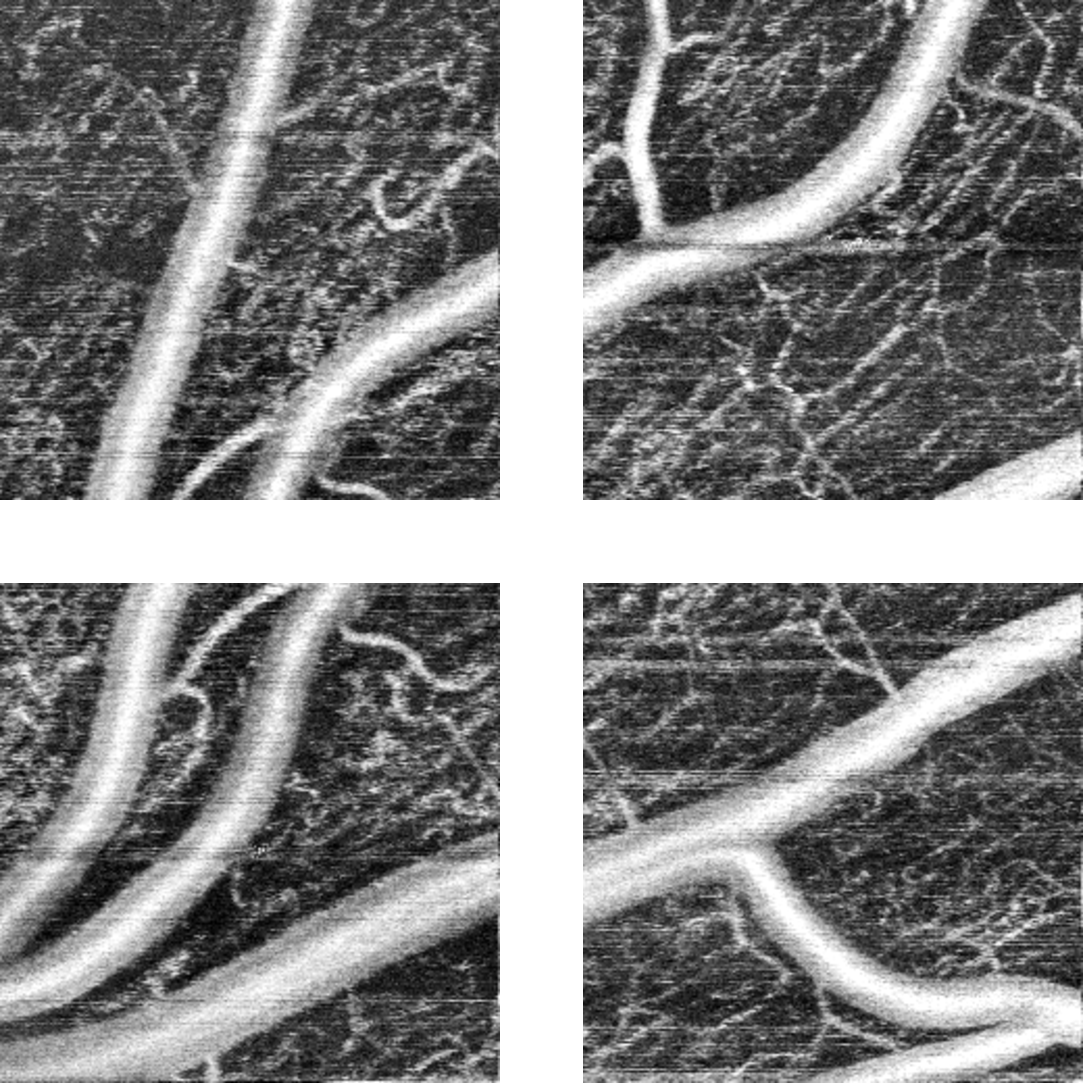
\includegraphics[width=5cm]{gfx/zbior_1}
  \caption{Przykładowy zbiór angiograficznych obrazów OCT umieszczonych zgodnie z ich współrzędnymi. Obraz referencyjny znajduje się w prawym górnym rogu.}
  \label{fig:wyniki_eksperymentow:zbior_1}
\end{figure}

\begin{figure}[htb]
  \centering
  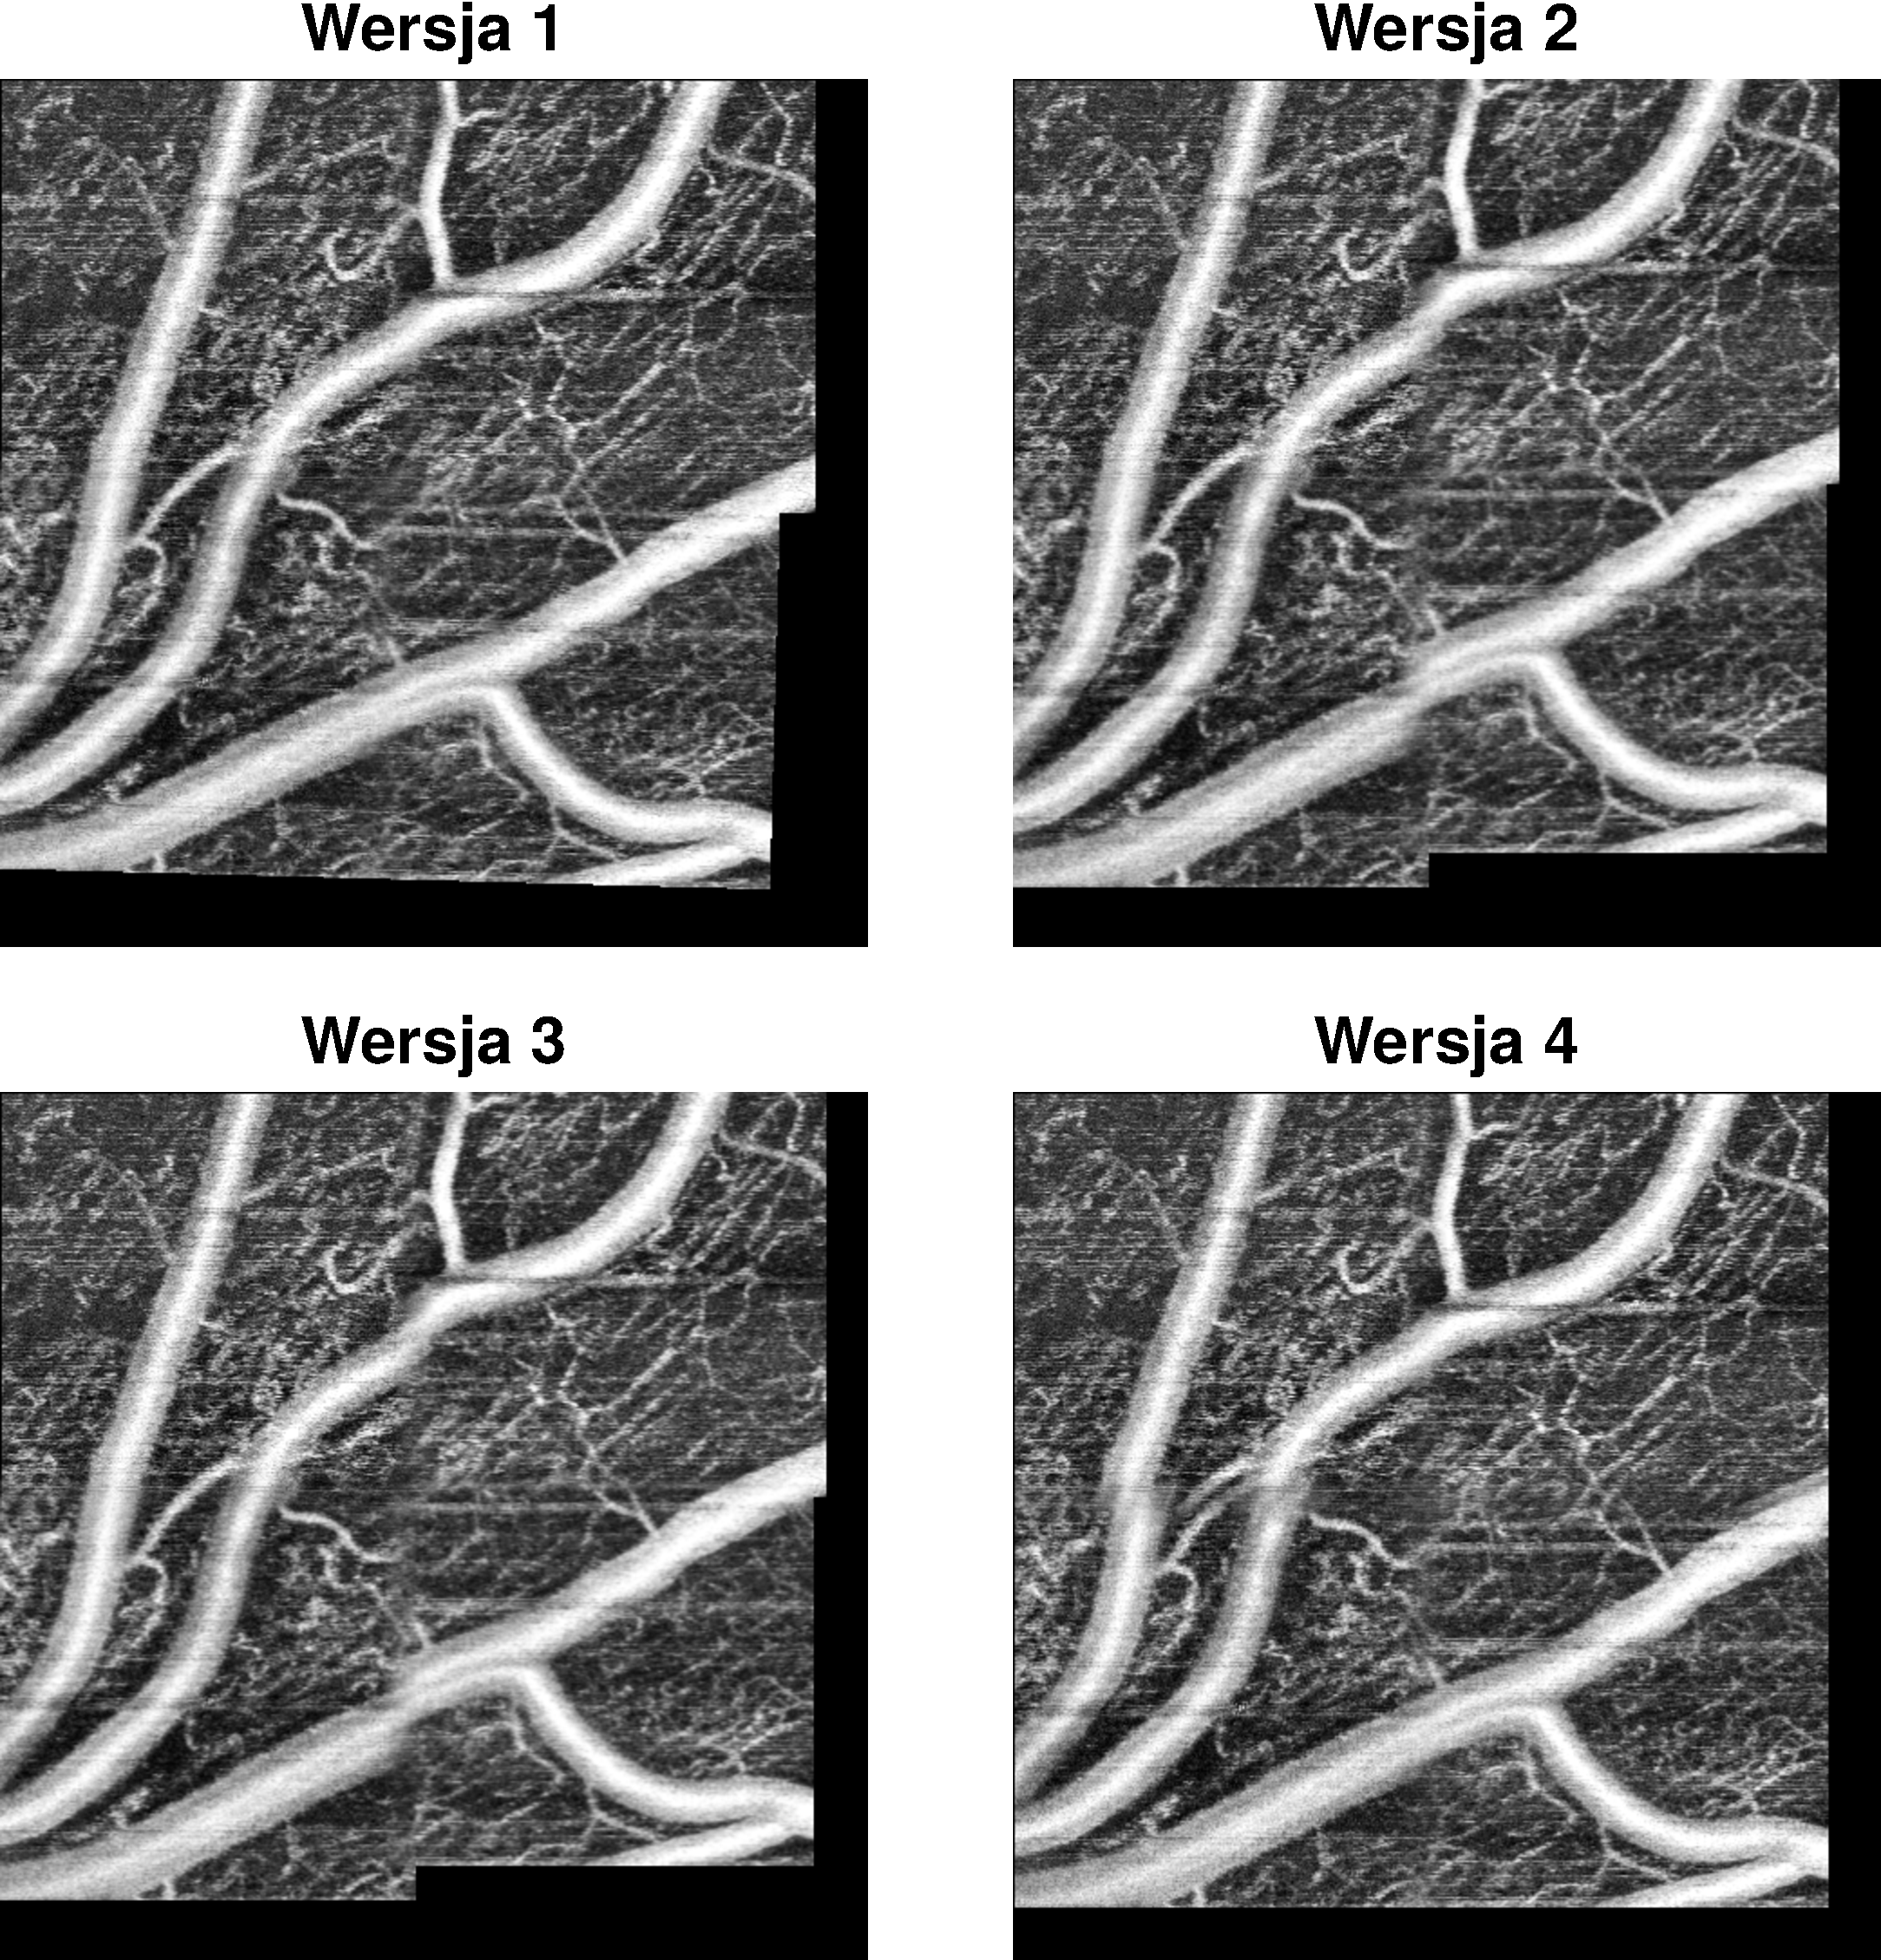
\includegraphics[width=10cm]{gfx/wynik_zbior_1}
  \caption{Cztery mozaiki będą wynikiem działania programu \texttt{mostitch} na zbiorze obrazów OCT z rysunku \ref{fig:wyniki_eksperymentow:zbior_1}.}
  \label{fig:wyniki_eksperymentow:wynik_zbior_1}
\end{figure}

\section{Zbiór 2}
\label{sec:zbior_2}

Rysunek \ref{fig:wyniki_eksperymentow:zbior_2} przedstawia zbiór angiograficznych obrazów OCT, natomiast rysunek \ref{fig:wyniki_eksperymentow:wynik_zbior_2} przedstawia wynik działania programu \texttt{mostitch}.

\begin{figure}[H]
  \centering
  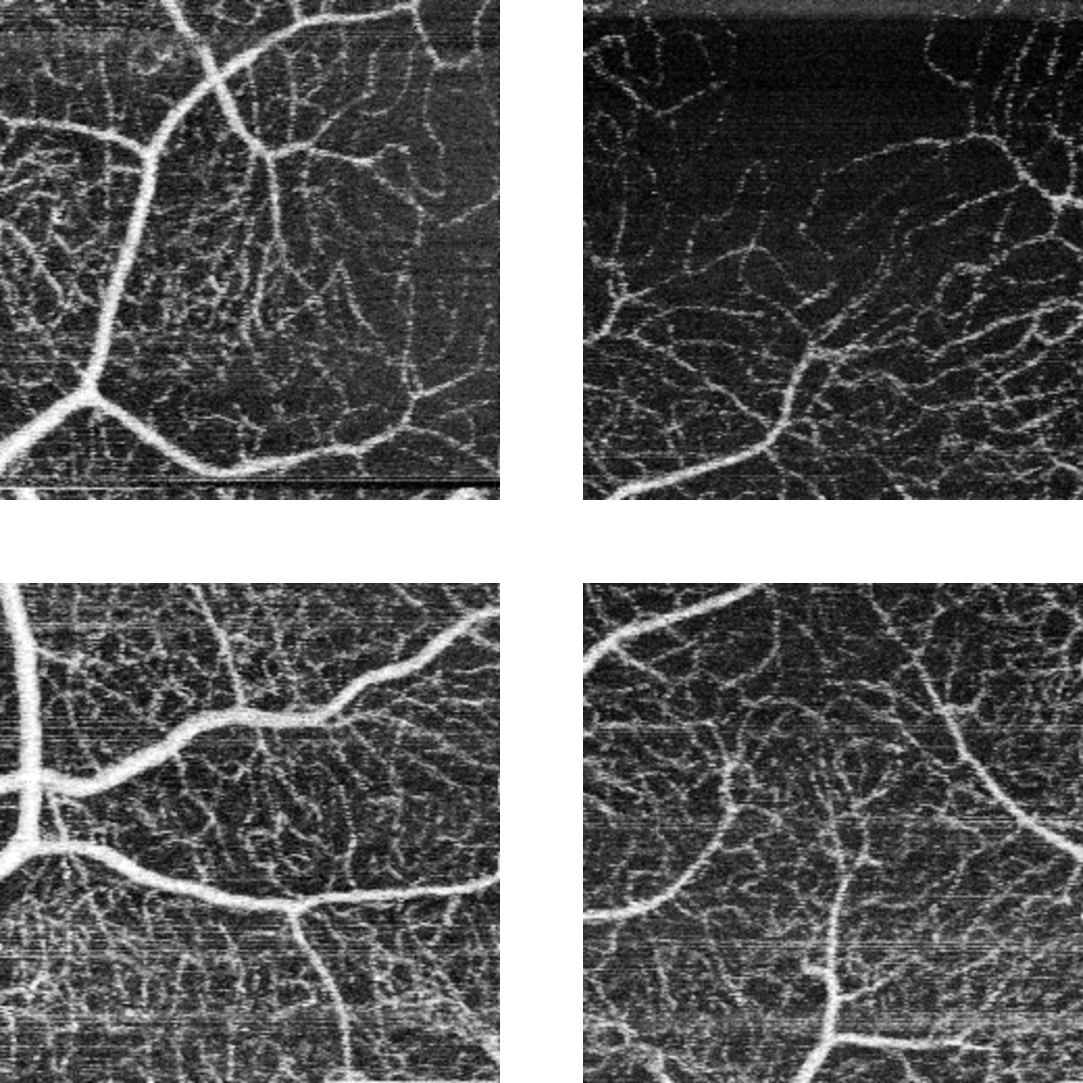
\includegraphics[width=5cm]{gfx/zbior_2}
  \caption{Przykładowy zbiór angiograficznych obrazów OCT umieszczonych zgodnie z ich współrzędnymi. Obraz referencyjny znajduje się w prawym górnym rogu.}
  \label{fig:wyniki_eksperymentow:zbior_2}
\end{figure}

\begin{figure}[htb]
  \centering
  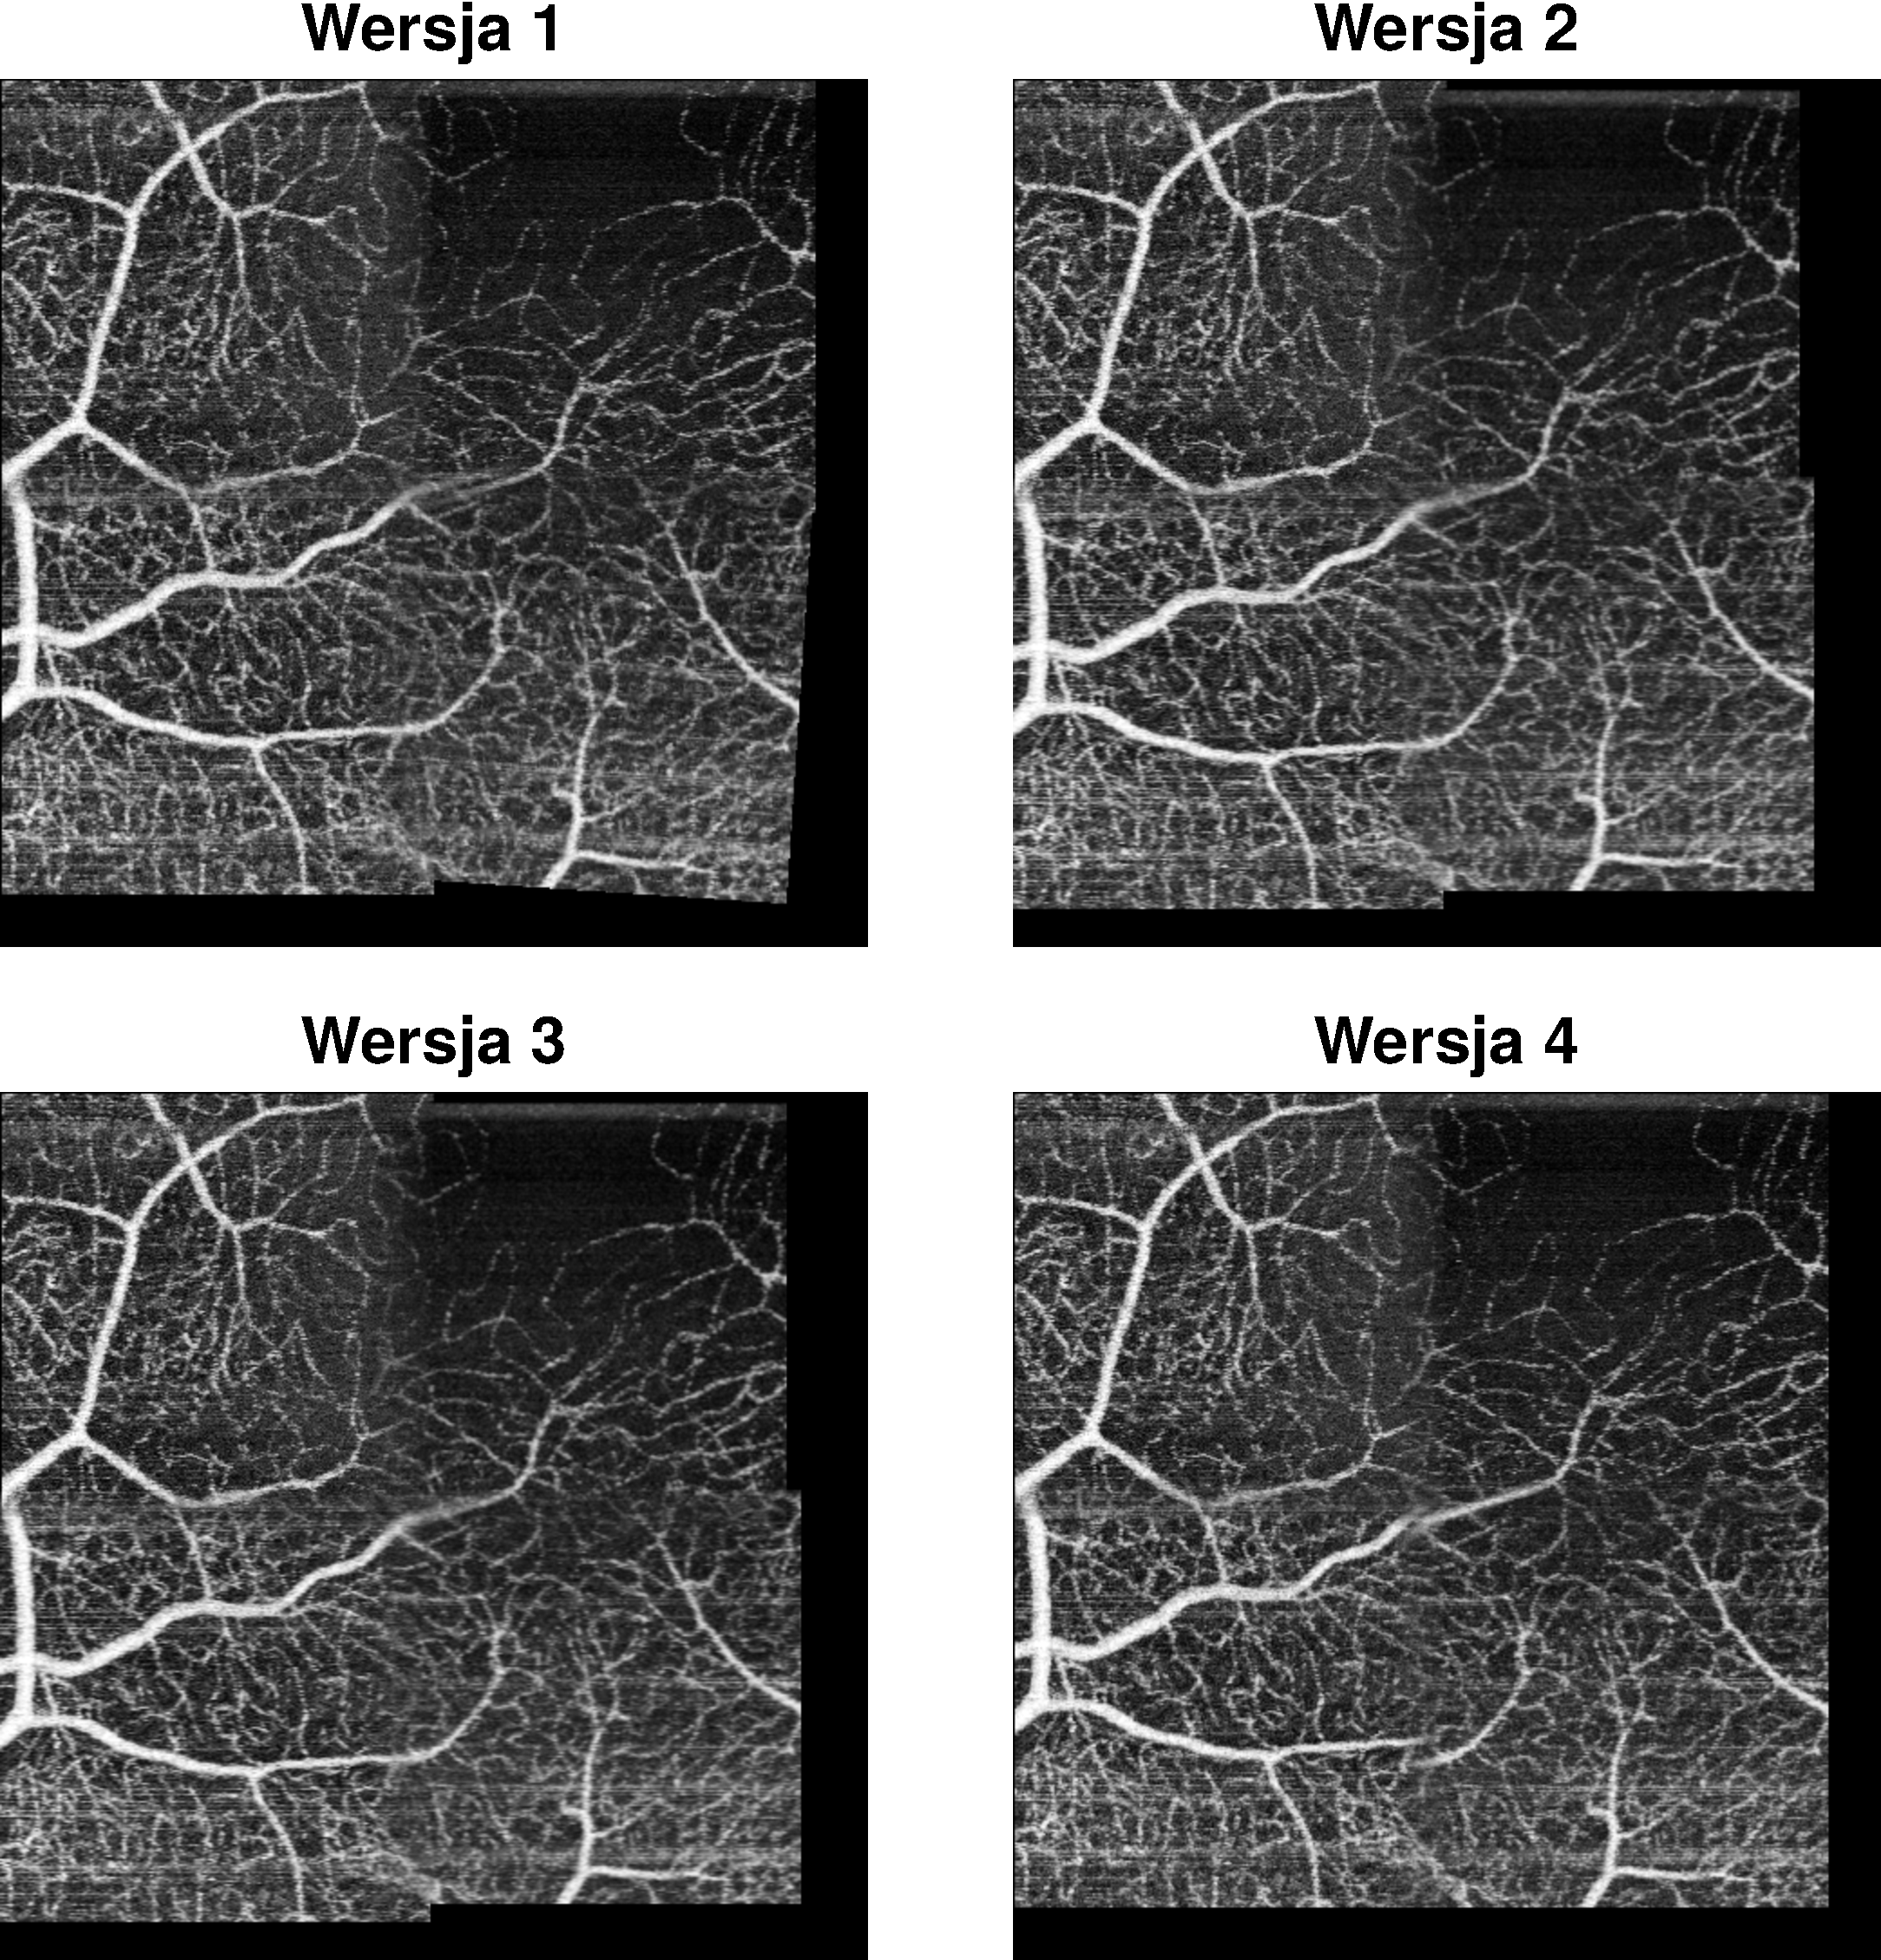
\includegraphics[width=10cm]{gfx/wynik_zbior_2}
  \caption{Cztery mozaiki będą wynikiem działania programu \texttt{mostitch} na zbiorze obrazów OCT z rysunku \ref{fig:wyniki_eksperymentow:zbior_2}.}
  \label{fig:wyniki_eksperymentow:wynik_zbior_2}
\end{figure}

\section{Zbiór 3}
\label{sec:zbior_3}

Rysunek \ref{fig:wyniki_eksperymentow:zbior_3} przedstawia zbiór angiograficznych obrazów OCT, natomiast rysunek \ref{fig:wyniki_eksperymentow:wynik_zbior_3} przedstawia wynik działania programu \texttt{mostitch}.

\begin{figure}[H]
  \centering
  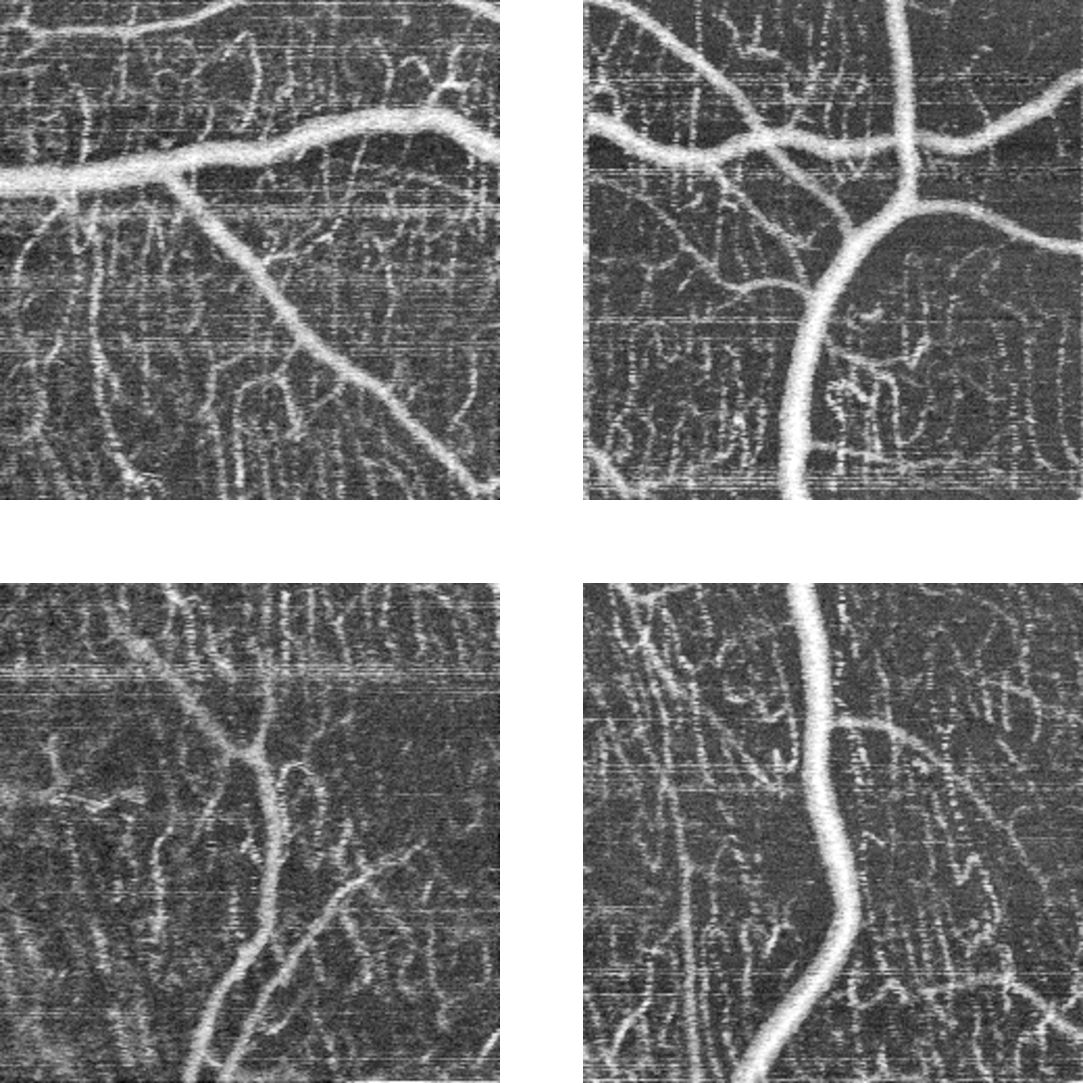
\includegraphics[width=5cm]{gfx/zbior_3}
  \caption{Przykładowy zbiór angiograficznych obrazów OCT umieszczonych zgodnie z ich współrzędnymi. Obraz referencyjny znajduje się w prawym górnym rogu.}
  \label{fig:wyniki_eksperymentow:zbior_3}
\end{figure}

\begin{figure}[htb]
  \centering
  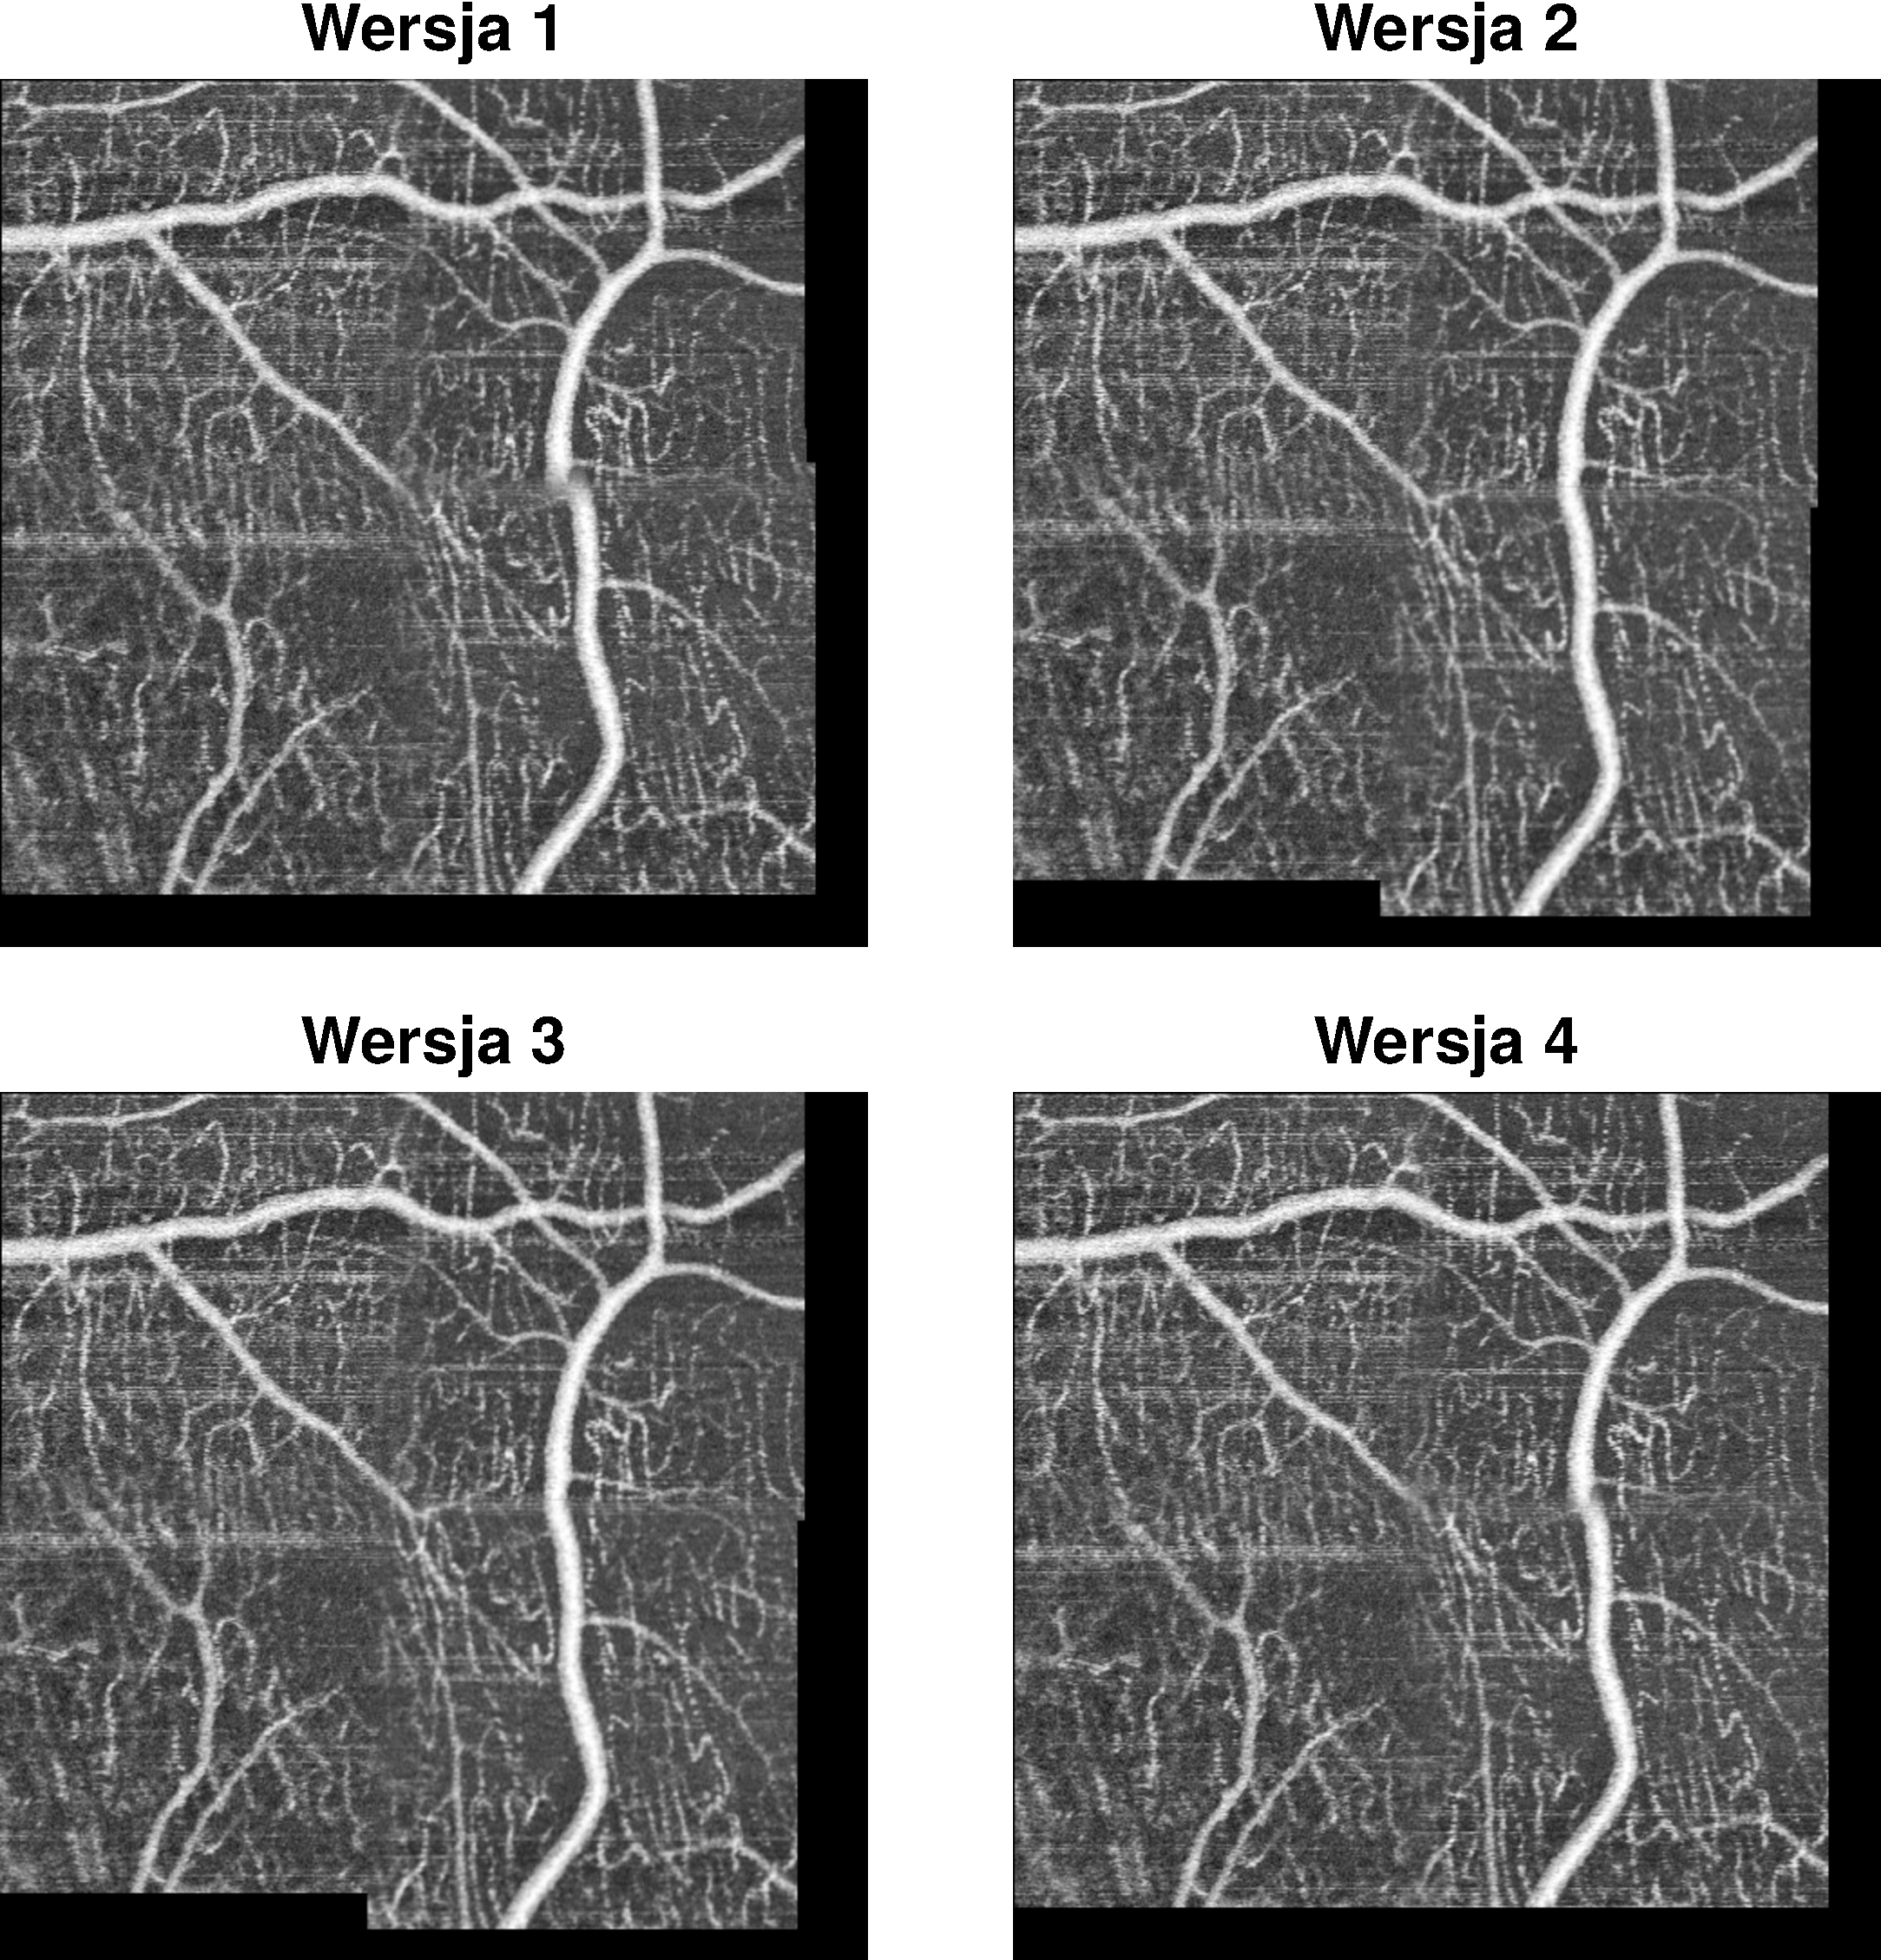
\includegraphics[width=10cm]{gfx/wynik_zbior_3}
  \caption{Cztery mozaiki będą wynikiem działania programu \texttt{mostitch} na zbiorze obrazów OCT z rysunku \ref{fig:wyniki_eksperymentow:zbior_3}.}
  \label{fig:wyniki_eksperymentow:wynik_zbior_3}
\end{figure}

\section{Ocena wyników}
\label{sec:ocena_wynikow}

W niniejszej sekcji przeprowadzono analizę wyników rozpoczynając od oceny wizualnej `na oko` w sekcji \ref{sec:wyniki_eksperymentow:ocena_wizualna}, następnie mozaiki oceniano poprzez policzenie odchylenia standardowego w miejscach nałożenia kafelków w sekcji \ref{sec:wyniki_eksperymentow:ochylenie_standardowe}. Czas wykonywania programu \texttt{mostitch} przedstawiono w sekcji \ref{sec:wyniki_eksperymentow:czas_wykonywania}. Na koniec podsumowano wyniki w sekcji \ref{sec:wyniki_eksperymentow:podsumowanie}.

\subsection{Ocena wizualna}
\label{sec:wyniki_eksperymentow:ocena_wizualna}

Na podstawie zaprezentowanych wyników dla trzech przykładowych zbiorów trudno wybrać wersję sprawdzającą się najlepiej dla każdego zbioru. Dla zbioru pierwszego z sekcji \ref{sec:zbior_1} najlepszą wersją jest wersja pierwsza, natomiast dla zbioru drugiego z sekcji \ref{sec:zbior_2} najlepiej prezentującym się wynikiem jest wersja druga lub trzecia. Dla zbioru trzeciego z sekcji \ref{sec:zbior_3} najlepiej wygląda mozaika stworzona wersją drugą lub trzecią. 

\subsection{Ocena na podstawie odchylenia standardowego}
\label{sec:wyniki_eksperymentow:ochylenie_standardowe}

Chcąc stworzyć wiarygodną miarę jakości końcowej mozaiki trzeba najpierw zdefiniować wzorzec, czyli mozaikę złożoną idealnie. W przypadku tematu niniejszej pracy definicja takiego wzorca jest problemem nietrywialnym ze względu na unikalne artefakty występujące w obrazach. Nie jest możliwym by nałożyć kafelki na siebie w taki sposób by piksele idealnie się pokrywały pod względem wartości. Z tego względu końcowa jakość mozaiki $Q$ to suma odchyleń standardowych wartości pikseli w $n$ miejscach gdzie kafelki nakładają się na siebie w mozaice:

\begin{equation}
Q = \sum_{i=1}^{n} \sigma_{i}
\label{eq:standard_deviation}
\end{equation}

Gdzie $\sigma_{i}$ to wartość odchylenia standardowego wartości pikseli kafelków nakładających się w miejscu $i$. Wykres na rysunku \ref{fig:wyniki_eksperymentow:odchylenie_standardowe} przedstawia wartość jakości finalnych mozaik przedstawionych w niniejszym rozdziale dla czterech wersji tworzenia mozaiki.

\begin{figure}[htb]
  \centering
  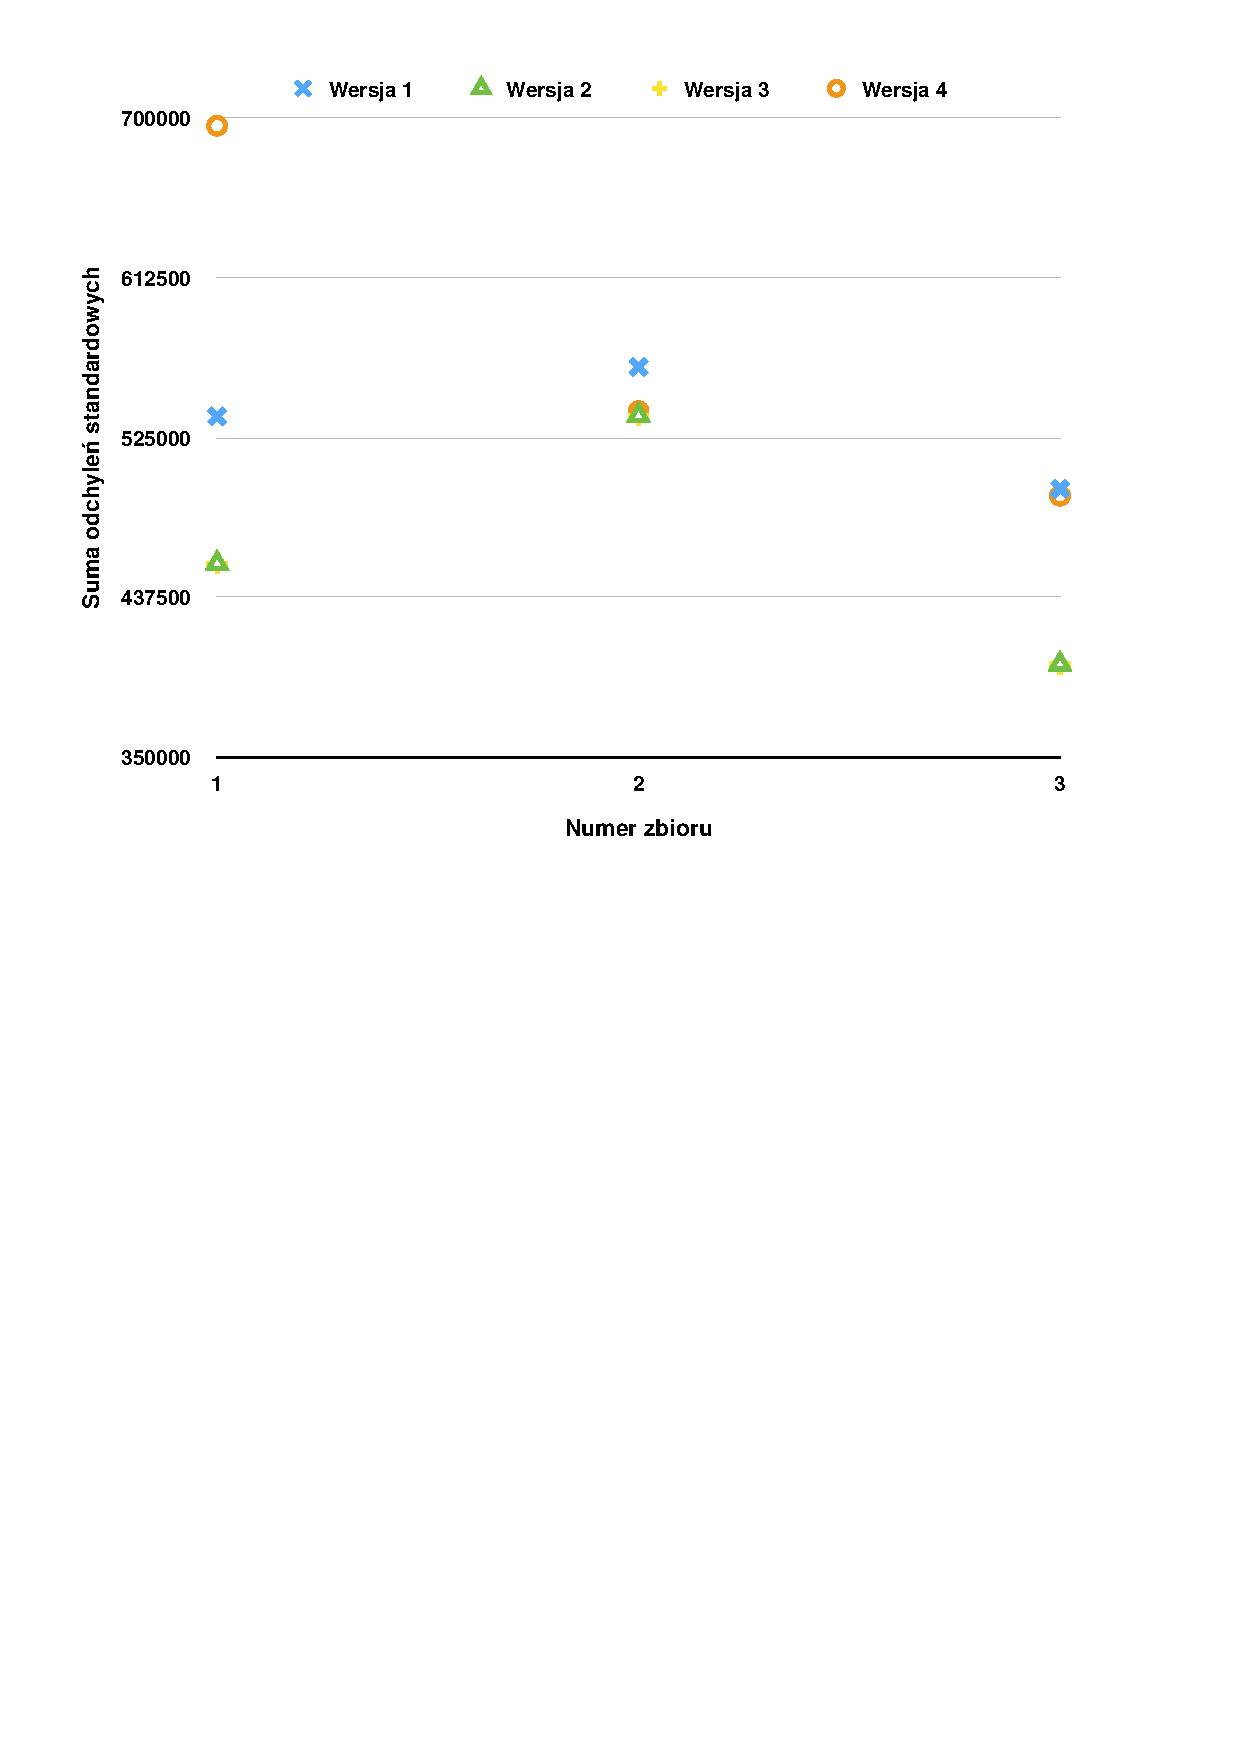
\includegraphics[width=\textwidth]{gfx/odchylenie_standardowe}
  \caption{Jakość finalnych mozaik przedstawionych w sekcjach \ref{sec:zbior_1}, \ref{sec:zbior_2} i \ref{sec:zbior_3} (im mniej tym lepiej).}
  \label{fig:wyniki_eksperymentow:odchylenie_standardowe}
\end{figure}

Wartości jakości odzwierciedlają ocenę wizualną (sekcja \ref{sec:wyniki_eksperymentow:ocena_wizualna}) za wyjątkiem zbioru pierwszego. Warto również zauważyć, że dla każdego zbioru wersja druga i trzecia zwracają najmniejszą (najlepszą) wartość jakości oraz jest to taka sama wartość. Wersja druga i trzecia różni się występowaniem w procesie algorytmu detekcji naczyń krwionośnych (sekcja \ref{sec:proponowane_algorytmy:depth_first_search}). W wersji drugiej, w której występuje, algorytm najwyraźniej nie zwrócił macierzy transformacji na podstawie wykrytych naczyń krwionośnych, przez co wersja druga jest identyczna do wersji trzeciej (proces dokładniej opisano w sekcji \ref{sec:proponowane_algorytmy:proces_decyzyjny}).

\subsection{Ocena na podstawie czasu wykonywania}
\label{sec:wyniki_eksperymentow:czas_wykonywania}

Wykres na rysunku \ref{fig:wyniki_eksperymentow:czas_wykonywania} przedstawia czas wykonywaniu programu \texttt{mostitch} na zbiorach przedstawionych w niniejszym rozdziale dla czterech wersji tworzenia mozaiki.

\begin{figure}[htb]
  \centering
  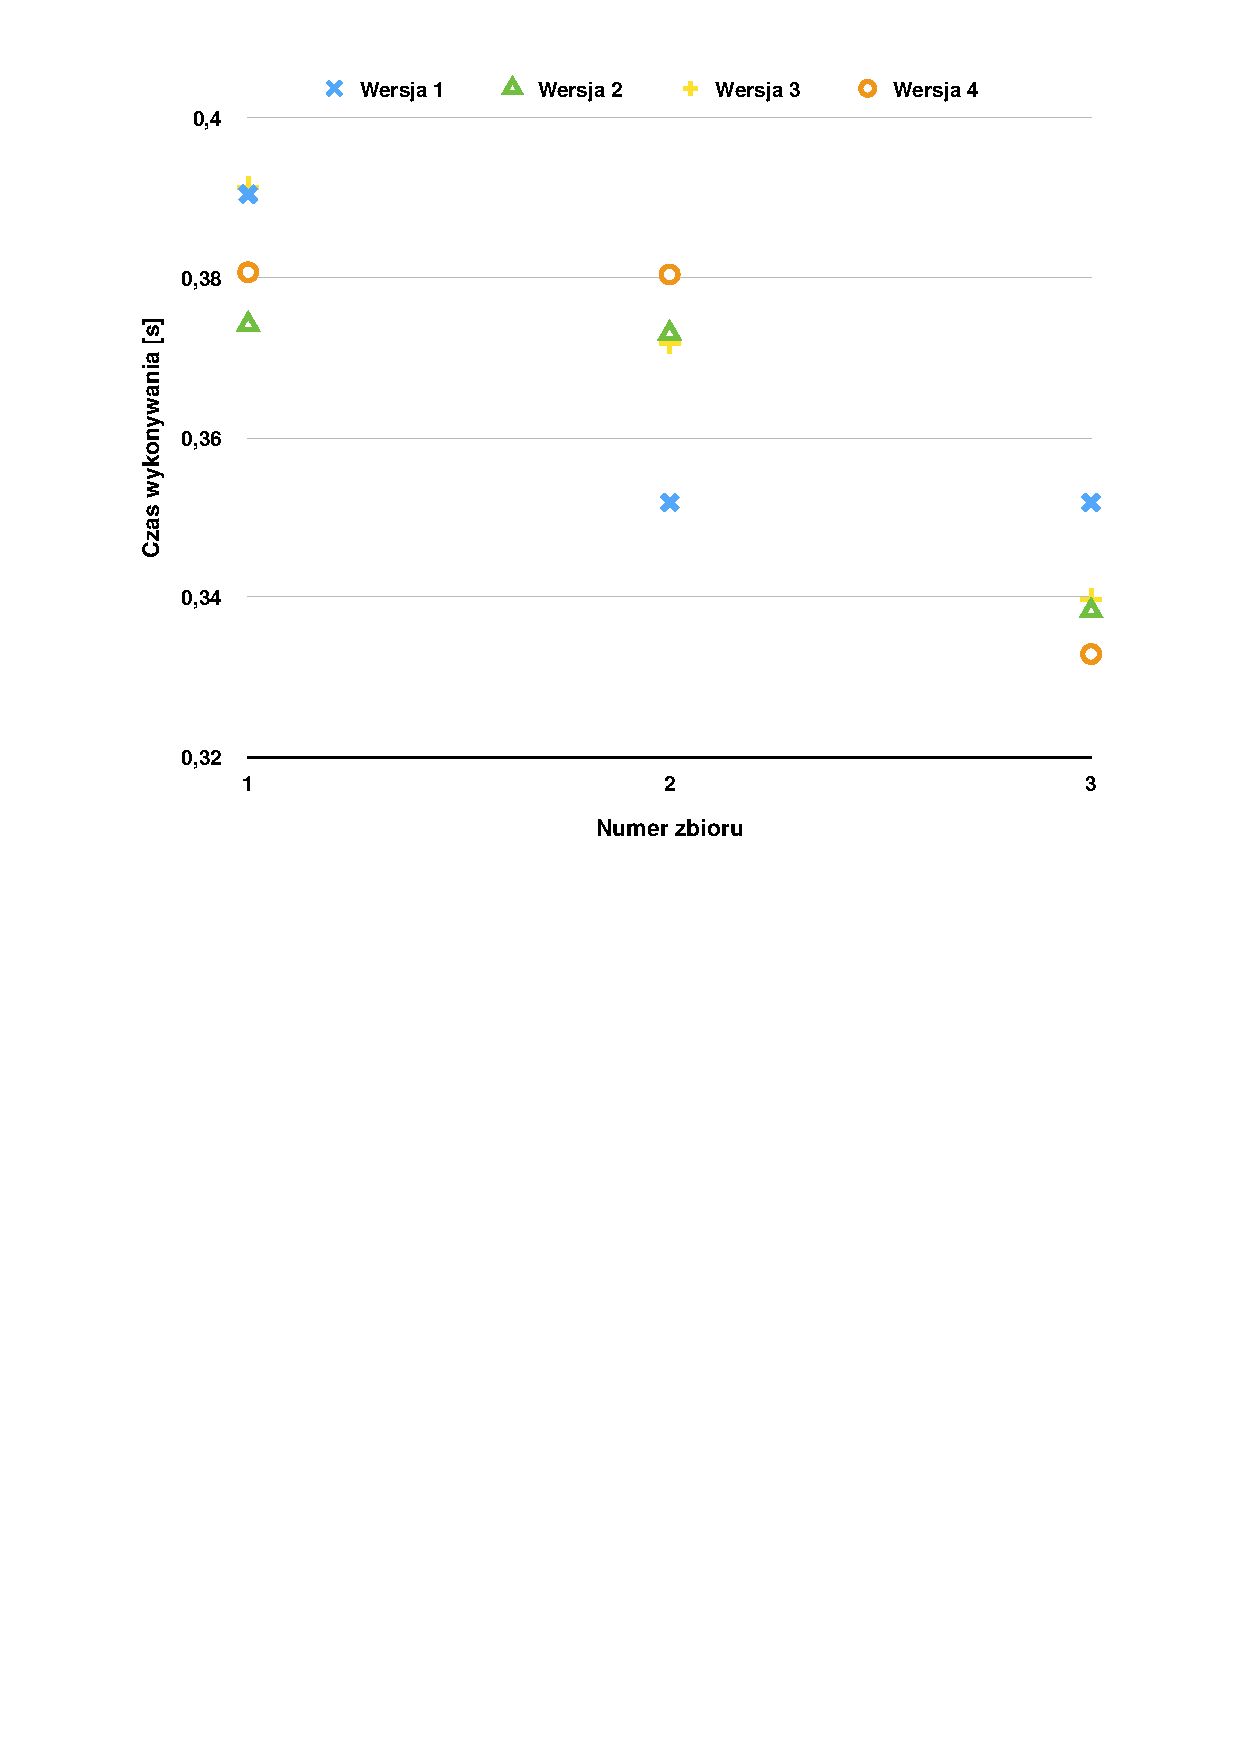
\includegraphics[width=\textwidth]{gfx/czas_wykonywania}
  \caption{Czas wykonywania programu \texttt{mostitch} na zbiorach przedstawionych w sekcjach \ref{sec:zbior_1}, \ref{sec:zbior_2} i \ref{sec:zbior_3}.}
  \label{fig:wyniki_eksperymentow:czas_wykonywania}
\end{figure}

Program \texttt{mostitch} najszybciej ($0,332853s$) stworzył mozaikę ze zbioru trzeciego za pomocą wersji czwartej. Na podstawie wyników zaprezentowanych na rysunku \ref{fig:wyniki_eksperymentow:czas_wykonywania} ciężko wybrać wersję, która jest najszybsza, albo najwolniejsza. Wynika to z tego, że dla każdej wersji większość skomplikowanych obliczeń pomimo ustawionych parametrów jest wykonywana. Jest to cecha programu, która na pewno może być ulepszona w przyszłości. Czasy wykonywania programu pomiędzy różnymi zbiorami również są bardzo podobne. Ta kwestia nie powinna dziwić, ponieważ każdy kafelek jest tego samego rozmiaru oraz posiada podobną ilość danych. 

\subsection{Podsumowanie}
\label{sec:wyniki_eksperymentow:podsumowanie}

Podsumowując analiza wizualna (sekcja \ref{sec:wyniki_eksperymentow:ocena_wizualna}), oraz analiza na podstawie czasu wykonania (sekcja \ref{sec:wyniki_eksperymentow:czas_wykonywania}) nie wyznaczyły jednoznacznie wersji, która osiąga najlepsze rezultaty. Analiza z wykorzystaniem odchylenia standardowego (sekcja \ref{sec:wyniki_eksperymentow:ochylenie_standardowe}) wyłoniła na faworytów wersję drugą oraz trzecią, natomiast pomyliła się co do zbioru pierwszego wskazując wersję drugą jako najlepszą, gdzie bezkonkurencyjnie wersja pierwsza stworzyła najlepszą mozaikę. Na podstawie trzech przeprowadzonych analiz nie jest możliwym wyłonić najlepszą wersję. Rozbieżność rezultatów dla różnych wartości parametrów jest głównym powodem tworzenia czterech różnych wersji mozaik przez program \texttt{mostitch}. Dzięki takiemu rozwiązaniu osoba z wiedzą ekspercką jest w stanie stwierdzić, który obraz nadaje się najlepiej do wybranego zastosowania. Co więcej, otrzymanie czterech różnych wynikowych mozaik oszczędza czas uruchamiania programu z różnymi wartościami parametrów.













